% !TeX TS-program = xelatex



\documentclass[]{beamer}
\usetheme{Madrid}
\usecolortheme{dolphin}

\usepackage{fontspec, xunicode, xltxtra}
\usepackage{amsmath, amsfonts, amssymb}
\usepackage{mathptmx}
\usepackage{graphicx}
\usepackage{epstopdf}
\usepackage{subfigure}
\usepackage[english]{babel}
\usepackage{tikz}
\usepackage{mathdots}
\usepackage{yhmath}
\usepackage{cancel}
\usepackage{color}
\usepackage{siunitx}
\usepackage{array}
\usepackage{multirow}
\usepackage{amssymb}
\usepackage{gensymb}
\usepackage{tabularx}
\usetikzlibrary{fadings}

\usepackage{algorithm}
\usepackage{algpseudocode}

\setmonofont{Courier New}

\renewcommand{\algorithmicrequire}{\textbf{Input:}} 
\renewcommand{\algorithmicensure}{\textbf{Output:}}

%\renewcommand{\vec}{\mathbf}
\setlength{\parskip}{0.2cm}

\usepackage{natbib}
\bibliographystyle{plain}

\title[VSA in Program Synthesis]{Version Space Algebra in Program Synthesis}
\institute[SPAR PL4SE]{SPAR PL4SE, Institute of Computer Software, Nanjing University}
\author{Shaoyuan Chen}
\date{March 12, 2020}


\begin{document}
\begin{frame}
	\titlepage
\end{frame}


\begin{frame}
	\frametitle{Version Space}
	In machine learning, the \textbf{version space method} proposed by Mitchell \cite{mitchell} learns a Boolean function from given positive/negative examples. Lau et. al. extended Mitchell's version space concept to functions with arbitrary range and defined \textbf{version space algebra} \cite{lau}. Using these techniques, they developed SMARTedit, a \textit{programming by demonstration} application for repetitive text editing tasks.
	
	\pause
	
	Version space algebra is especially useful in
	\begin{enumerate}
		\item programming by demonstration (PbD);
		\item synthesizing action sequences (e.g., text-editing scripts \cite{mitchell}, robot control programs \cite{pardowitz}).
	\end{enumerate}
	It can even be used to synthesize shell scripts \cite{shell} and simple python programs \cite{python}.
\end{frame}

\begin{frame}
\frametitle{Terminology}
\begin{description}
	\item[Hypothesis] a function (from attribute space to label space) in machine learning; a program (from input space to output space) in program synthesis. 
	\item[Hypothesis space] the set of all functions can be learned by a learning algorithm; the set of all programs can be produced by a synthesizer (= search space).
	\item[Version Space] the set of all hypotheses in a hypothesis space $H$ consistent with all training examples in a training set $D$, referred as $VS_{H, D}$. 
\end{description}
\end{frame}

\begin{frame}
\frametitle{Example: Binary Classification with Rectangle }
Problem: given a set of points with binary labels in a plane, find a rectangle that separates all positive points and all negative sample points.
\pause
\begin{itemize}
\item Hypothesis: all functions $h: \mathbb{R}^2 \rightarrow \{0, 1\}$
\item Hypothesis space: $\{h | \{(x, y): h(x, y) = 1\} = [A, B] \times [C, D]\}$
\end{itemize}
\pause
	\begin{figure}[h]
		\centering
		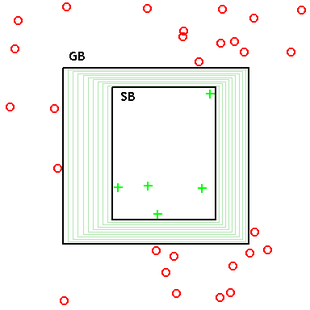
\includegraphics[width=4cm]{rect.png}
	\end{figure}
\end{frame}


\begin{frame}
	\frametitle{Candidate Elimination Algorithm}
	The \textit{candidate elimination algorithm} is used to compute the version space $VS_{H,D}$ given hypothesis space $H$ and training set $D$.
	\begin{algorithm}[H] 
		\caption{Candidate elimination algorithm} 
		\begin{algorithmic}[1] 
			\Require hypothesis space $H$; training set $D$
			\Ensure version space $VS_{H, D}$
			\State $VS \leftarrow H$
			\For {each training sample $(x, y)$ in $D$}
			\State $VS \leftarrow \{h \in VS | h(x) = y\}$ \Comment Refinement step
			\EndFor
			\State \Return $VS$
		\end{algorithmic} 
	\end{algorithm}
	\pause
	Maintaining the version space as a list of hypotheses is often infeasible, because the size of the hypothesis space may be very large. We need to find a \textit{compressed} representation of a version space to speed up the refinement step.
\end{frame}

\begin{frame}
\frametitle{Hypotheses Space as a Poset}
We may define a partial order between the hypotheses in a hypothesis space.

For Boolean-valued functions, a canonical partial order has been defined.

\begin{definition}[generality order]
	For hypotheses with Boolean values, we say $h_1$ is \textbf{more general} than $h_2$ $(h_1 \succeq h_2)$ if $h_2(x) \rightarrow h_1(x)$ for all $x$ in input space. The induced partial order in a hypothesis space is called the \textbf{generality order}.
\end{definition}

For arbitrary-valued functions, the partial order may be defined by the application designer.

\end{frame}

\begin{frame}
	\frametitle{Example: the ``ab?" Language}
	\begin{itemize}
	\item Hypothesis: $\{a, b\}^2 \rightarrow \{0, 1\}$
	
	\item Hypothesis space: $\{a, b, ?\}^2$, where ? matches any character 
	
	\item Hasse diagram of the generality order:
	
	\begin{figure}[h]
		
		\tikzset{every picture/.style={line width=0.75pt}} %set default line width to 0.75pt        
		
		\centering
		
		\begin{tikzpicture}[x=0.75pt,y=0.75pt,yscale=-1,xscale=1]
		%uncomment if require: \path (0,310); %set diagram left start at 0, and has height of 310
		
		%Shape: Rectangle [id:dp825214924085774] 
		\draw   (91,7.5) -- (121,7.5) -- (121,27.5) -- (91,27.5) -- cycle ;
		%Shape: Rectangle [id:dp3776116743100961] 
		\draw   (16,56.5) -- (46,56.5) -- (46,76.5) -- (16,76.5) -- cycle ;
		%Shape: Rectangle [id:dp1256361658218439] 
		\draw   (66,57) -- (96,57) -- (96,77) -- (66,77) -- cycle ;
		%Shape: Rectangle [id:dp6880517692458941] 
		\draw   (116,57.5) -- (146,57.5) -- (146,77.5) -- (116,77.5) -- cycle ;
		%Shape: Rectangle [id:dp9032367868304563] 
		\draw   (166,58) -- (196,58) -- (196,78) -- (166,78) -- cycle ;
		%Shape: Rectangle [id:dp4397455344406429] 
		\draw   (16,105) -- (46,105) -- (46,125) -- (16,125) -- cycle ;
		%Shape: Rectangle [id:dp2692781951495262] 
		\draw   (66,105.5) -- (96,105.5) -- (96,125.5) -- (66,125.5) -- cycle ;
		%Shape: Rectangle [id:dp22897577978882255] 
		\draw   (116,106) -- (146,106) -- (146,126) -- (116,126) -- cycle ;
		%Shape: Rectangle [id:dp8007111188673706] 
		\draw   (166,106.5) -- (196,106.5) -- (196,126.5) -- (166,126.5) -- cycle ;
		%Straight Lines [id:da9599802605350887] 
		\draw    (104.39,27.97) -- (32.39,55.97) ;
		%Straight Lines [id:da8367158246776023] 
		\draw    (104.39,27.97) -- (82.39,56.97) ;
		%Straight Lines [id:da553205185757548] 
		\draw    (104.39,27.97) -- (130.39,57.97) ;
		%Straight Lines [id:da7955379024277809] 
		\draw    (104.39,27.97) -- (182.39,57.97) ;
		%Straight Lines [id:da33064958726190574] 
		\draw    (31.39,75.97) -- (31.39,105.97) ;
		%Straight Lines [id:da2592184751600124] 
		\draw    (31.39,105.97) -- (131.39,76.97) ;
		%Straight Lines [id:da43779360233525955] 
		\draw    (31.39,75.97) -- (80.39,104.97) ;
		%Straight Lines [id:da07133648876619603] 
		\draw    (82.39,76.97) -- (131.39,105.97) ;
		%Straight Lines [id:da8139790755534921] 
		\draw    (81.39,76.97) -- (181.39,105.97) ;
		%Straight Lines [id:da27938653386600554] 
		\draw    (131.39,105.97) -- (131.39,76.97) ;
		%Straight Lines [id:da509802724282018] 
		\draw    (181.39,105.97) -- (181.39,76.97) ;
		%Straight Lines [id:da055380585839575724] 
		\draw    (80.39,104.97) -- (181.39,76.97) ;
		
		% Text Node
		\draw (106,17.5) node   [align=left] {??};
		% Text Node
		\draw (31,66.5) node   [align=left] {a?};
		% Text Node
		\draw (81,67) node   [align=left] {b?};
		% Text Node
		\draw (131,67.5) node   [align=left] {?a};
		% Text Node
		\draw (181,68) node   [align=left] {?b};
		% Text Node
		\draw (31,115) node   [align=left] {aa};
		% Text Node
		\draw (81,115.5) node   [align=left] {ab};
		% Text Node
		\draw (131,116) node   [align=left] {ba};
		% Text Node
		\draw (181,116.5) node   [align=left] {bb};
		
		
		\end{tikzpicture}
		
	\end{figure}
	
	\end{itemize}

\end{frame}

\begin{frame}
\frametitle{Boundary-Set Representability}
With a partial order defined on the hypothesis space, we may use two antichains $G$, $S$ (called \textit{boundaries}) to represent a version space.

\begin{definition}[boundary-set representability]
	A version space $VS$ of a partially-ordered hypothesis space $H$ is \textbf{boundary-set representable (BSR)}, if it can be written as the form
	$$
	VS = \{h \in H | \exists h_g \in G, \exists h_s \in S, h_g \succeq h \succeq h_s \}
	$$
	where $G$, $S$ are two antichains of $H$.
\end{definition}

\pause

Examples for the ``ab?" language: 
\begin{itemize}
	\item $D = \{(ab, 1)\}$: $G = \{??\}$, $S = \{ab\}$;
	\item $D = \{(aa, 0)\}$: $G = \{b?, ?a\}$, $S = \{ab, ba, bb\}$;
	\item $D = \{(aa, 1), (ab, 1)\}$: $G = S = \{a?\}$.
\end{itemize}

\end{frame}

\begin{frame}
\frametitle{Boundary-Set Representability}

Not all version spaces are BSR. Hirsh showed that \textbf{convexity} and \textbf{definiteness} are a necessary and sufficient condition for a version space being BSR \cite{hirsh}.
	
	A subset $C$ of a partially ordered set $(S, \preceq)$ is
	\begin{itemize}
		\item \textbf{convex}, if: $x \preceq y \preceq z$ $(x, z \in C, y \in S)$ implies $y \in C$;
		\item \textbf{definite}, if: for every $y \in C$, there exists $x \in \min\{C\}$ (minimal elements of $C$) and $z \in \max\{C\}$ (maximal elements of $C$), such that $x \preceq y \preceq z$.
	\end{itemize}

\pause

\begin{theorem}[version space representation theorem]
	Every version space of a Boolean hypothesis space with generality order is BSR.
\end{theorem}
\end{frame}

\begin{frame}
\frametitle{Boundary-Set Representability}

With boundary-set representation, the version space can be updated in a more efficient approach.

\pause

Example:
\begin{itemize}
\item Hypothesis: $\Sigma^* \rightarrow \{0, 1\}$ where $\Sigma = \{a,b,c\})$
\item Hypothesis space: $\{ s* | s \in \Sigma^*\}$
\end{itemize}

\pause

\begin{enumerate}[<+->]
	\item $D = \{(\text{aba}, 1)\}$, $G = \{*\}$, $S = \{aba*\}$;
	\item $D = \{(\text{aba}, 1), (\text{ba}, 0)\}$, $G = \{a*\}$, $S = \{aba*\}$;
	\item $D = \{(\text{aba}, 1), (\text{ba}, 0), (\text{abc}, 1)\}$, $G = \{a*\}$, $S = \{ab*\}$;
\end{enumerate}

\end{frame}

\begin{frame}
\frametitle{Version Space Algebra}

Lau et. al. defined \textbf{version space algebra}, which allows us to build complex version space from simple, atomic version spaces.

\pause 

\begin{definition}[version space union]
	Given two hypothesis spaces $H_1, H_2$ with the same input and output spaces, the \textbf{union} of two version spaces $VS_{H_1, D} \cup VS_{H_2, D}$ is defined as $VS_{H_1 \cup H_2, D}$ .
\end{definition}

\begin{definition}[version space join]
	Given two version spaces $VS_{H_1, D_1}$ and $VS_{H_2, D_2}$, the \textbf{independent join} of the two spaces $VS_{H_1, D_1} \bowtie VS_{H_2, D_2}$ is defined as $$\{\langle h_1, h_2 \rangle| h_1 \in VS_{H_1, D_1}, h_2 \in VS_{H_2, D_2}\},$$
	where
	$ \langle h_1, h_2 \rangle (x, y) \equiv (h_1(x), h_2(y))$.
\end{definition}

\end{frame}

\begin{frame}
	\frametitle{Version Space Algebra}
	The version space algebra is analogous to the context-free grammar, in the following sense:
	\begin{table}[h]
		\centering
	\begin{tabular}{|c|c|}
		\hline 
		\textbf{VSA} & \textbf{CFG} \\ 
		\hline 
		atomic version space & terminal symbol \\ 
		compound version space & non-terminal symbol \\ 
		version space union & ``or'' of two production rules \\ 
		version space join & concatenation of two symbols \\ 
		\hline 
	\end{tabular} 
	\end{table}

	Note: compound version spaces can be represented by representing all its components simultaneously; thus compound version space can be updated by updating all components individually.
\end{frame}

\begin{frame}
\frametitle{Example: SMARTedit}

\begin{figure}[h]
	\centering
	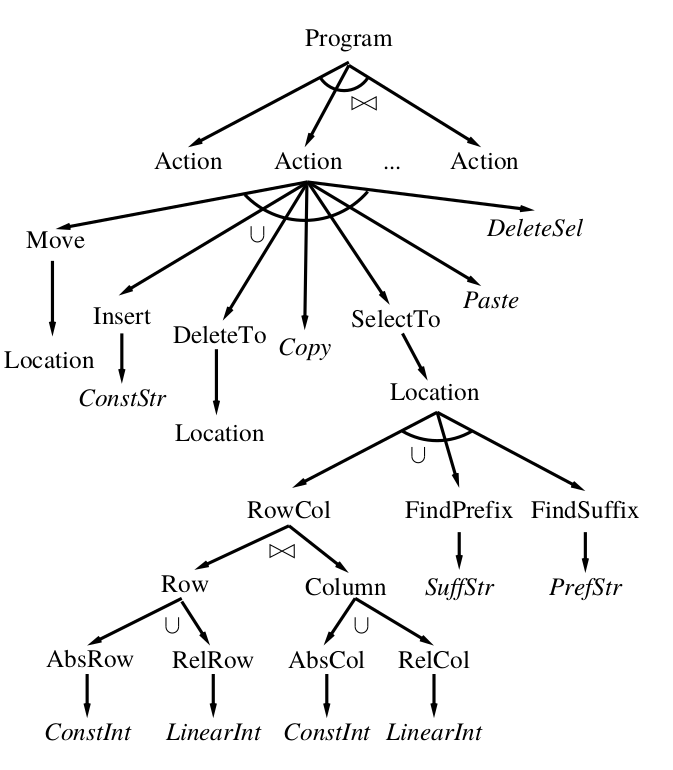
\includegraphics[width=6cm]{smartedit.png}
	\caption{Version space structure for SMARTedit}
\end{figure}

\end{frame}

\begin{frame}
	\frametitle{References}
	\bibliography{vsa}
\end{frame}

\end{document}

